\documentclass[11pt,a4paper]{article}
\usepackage[T1]{fontenc}
\usepackage[utf8]{inputenc}
\usepackage{lmodern,microtype}
\usepackage[margin=22mm,headheight=15pt]{geometry}
\usepackage{amsmath,amssymb,booktabs,tabularx,array,enumitem}
\usepackage{xcolor,tikz,fancyhdr,titlesec,hyperref}
\usetikzlibrary{arrows.meta,positioning,calc}
\definecolor{navy}{HTML}{193B54}
\definecolor{teal}{HTML}{087E8B}
\definecolor{pale}{HTML}{EDF6F6}
\definecolor{graycell}{HTML}{DCE1E5}
\hypersetup{colorlinks=true,linkcolor=navy,urlcolor=teal,citecolor=teal,
  pdftitle={AGFL-inm: Current research pipeline, dataset and training losses},
  pdfauthor={AGFL-inm research documentation}}
\pagestyle{fancy}\fancyhf{}
\fancyhead[L]{\small\textcolor{navy}{AGFL-inm\quad Current research guide}}
\fancyhead[R]{\small 2 October 2026}
\fancyfoot[C]{\thepage}
\setlength{\parindent}{0pt}\setlength{\parskip}{4pt}
\titlespacing*{\section}{0pt}{10pt}{6pt}
\titlespacing*{\subsection}{0pt}{8pt}{4pt}
\setlist{itemsep=3pt,topsep=4pt,leftmargin=*}
\renewcommand{\arraystretch}{1.12}
\newcolumntype{Y}{>{\raggedright\arraybackslash}X}
\newcolumntype{L}[1]{>{\raggedright\arraybackslash}p{#1}}
\newcommand{\code}[1]{{\small\nolinkurl{#1}}}
\newcommand{\takeaway}[1]{\par\smallskip\noindent\fcolorbox{teal}{pale}{%
  \parbox{\dimexpr\linewidth-2\fboxsep-2\fboxrule\relax}{#1}}\par\smallskip}
\tikzset{box/.style={draw=teal,fill=pale,rounded corners=2pt,align=center,
  text width=42mm,minimum height=14mm,font=\small,inner sep=4pt},
  arrow/.style={-{Latex[length=2mm]},thick,draw=navy}}

\begin{document}
{\LARGE\bfseries\color{navy} Current research pipeline}\par
{\large Dataset, EEG classification, and training losses}\par
\textbf{Scope:} branch \code{research/baseline-accuracy}, source revision
\code{4c27ec0}. Main example: \code{configs/baselines-reproducible.json}.

\section{What are we trying to learn?}
An EEG recording contains voltage measurements from electrodes on the scalp.
For each four-second trial, the model predicts which movement the participant
was \emph{imagining}: left hand, right hand, feet, or tongue. We also ask how
predictions change when some electrodes become unavailable.

Our immediate research direction is to understand a simple, reproducible
EEGNet baseline before adding more architecture. The broader question is whether
a tensor representation or completion method can improve robustness to electrode
loss. Those are related questions, but they require separate comparisons.

\begin{center}
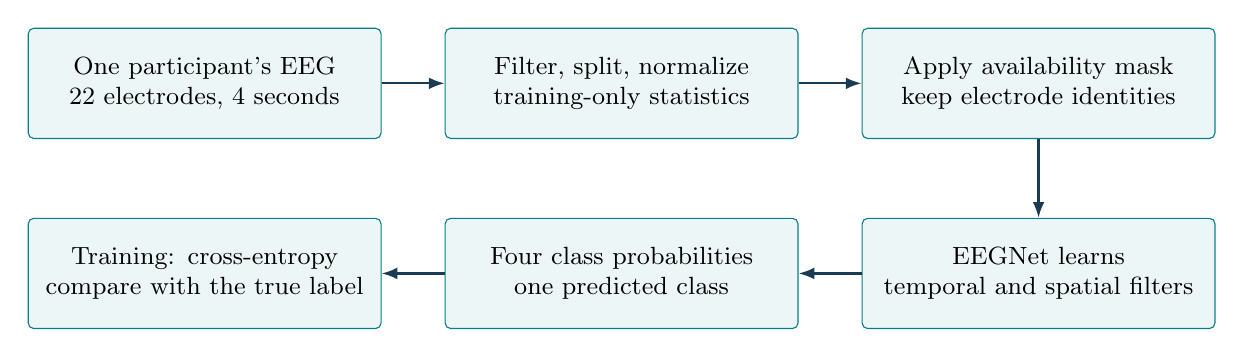
\begin{tikzpicture}[node distance=10mm and 8mm]
\node[box] (data) {One participant's EEG\\22 electrodes, 4 seconds};
\node[box,right=of data] (prep) {Filter, split, normalize\\training-only statistics};
\node[box,right=of prep] (mask) {Apply availability mask\\keep electrode identities};
\node[box,below=of mask] (net) {EEGNet learns\\temporal and spatial filters};
\node[box,left=of net] (prob) {Four class probabilities\\one predicted class};
\node[box,left=of prob] (loss) {Training: cross-entropy\\compare with the true label};
\draw[arrow] (data)--(prep);\draw[arrow] (prep)--(mask);
\draw[arrow] (mask)--(net);\draw[arrow] (net)--(prob);\draw[arrow] (prob)--(loss);
\end{tikzpicture}
\end{center}
\textbf{At prediction time, the true label is not an input.} Labels are needed
to train the model and later to score its predictions.

\subsection*{Three designs currently discussed in the project}
\begin{tabularx}{\linewidth}{@{}L{31mm}YY@{}}
\toprule
Design & What it does & Status in this guide \\
\midrule
Current accuracy baseline & Raw masking, end-to-end EEGNet; also a covariance reference & Main explanation, pages 2--6 \\
Earlier tensor pipeline & Frozen channel-local features, then tensor core/completion and attention & Explained separately on page 7 \\
George's redesign & Raw-signal completion before EEGNet or Signal Transformer, both with MHA & Separate branch at \code{92b7fc2}; page 7 \\
\bottomrule
\end{tabularx}

\takeaway{\textbf{The current baseline has no attention block and no Tucker
module.} Its convolutional feature extractor and classifier learn together from
class labels. Tensor reconstruction is a separate objective used only in the
tensor designs.}

\textbf{Reading order.} Dataset and timing: page 2. Preprocessing and missing
electrodes: page 3. Model architecture: page 4. Training loss: page 5.
Checkpoint selection and evaluation: page 6. Tensor losses: page 7.
Source map and references: page 8.

\newpage
\section{Dataset and the meaning of one trial}
\subsection*{The recording collection}
BCI Competition IV, dataset 2a contains nine participants, each recorded in two
sessions on different days. Each session has six runs of 48 trials: 288 trials,
nominally 72 per class. There are 22 EEG and three eye-movement (EOG) channels sampled at
250 Hz; our classifier uses only the EEG channels. The four imagery classes
are left hand, right hand, feet, and tongue \cite{dataset}.

\begin{tabularx}{\linewidth}{@{}L{42mm}Y@{}}
\toprule
Item & Meaning in our default baseline \\
\midrule
Input files & \code{A01T.gdf} through \code{A09T.gdf}; each participant is processed separately \\
Trial & 1000 samples starting at a class cue; $1000/250=4$ seconds \\
One input & $22\times1000$ numbers, or $22\times4\times250$ after reshaping \\
Target label & $y\in\{0,1,2,3\}$: left hand, right hand, feet, tongue \\
Excluded trials & Artifact-marked, out-of-bounds, or nonfinite after filtering; counts are saved \\
Actual sample count & Depends on exclusions; do not assume all 288 trials survive \\
\bottomrule
\end{tabularx}

\subsection*{Cue time is different from trial-start time}
In the recording paradigm, fixation starts at trial time 0, the movement cue
appears at 2 seconds, and imagery continues until 6 seconds \cite{dataset}.
Our extraction begins at the \emph{cue}, with zero additional offset.

\begin{center}
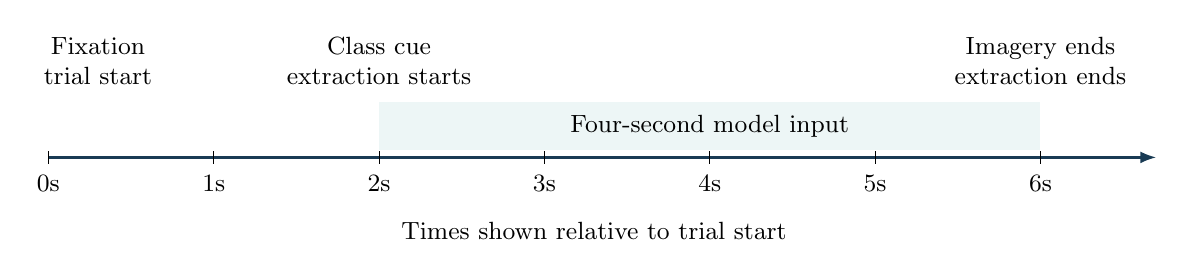
\begin{tikzpicture}[x=21mm,y=10mm,font=\small]
\fill[pale] (2,0.1) rectangle (6,0.7);
\draw[arrow] (0,0)--(6.7,0);
\foreach \t in {0,1,2,3,4,5,6}{\draw (\t,-.08)--(\t,.08);\node[below] at (\t,-.1){\t s};}
\node[above,align=center] at (.3,.8){Fixation\\trial start};
\node[above,align=center] at (2,.8){Class cue\\extraction starts};
\node[above,align=center] at (6,.8){Imagery ends\\extraction ends};
\node at (4,.4){Four-second model input};
\node[below] at (3.3,-.7){Times shown relative to trial start};
\end{tikzpicture}
\end{center}
The loader maps cue codes 769--772 to labels 0--3. It uses trial and run
boundaries to avoid extracting across recordings. Each accepted trial keeps a
stable ID so that its split membership and masks can be checked later.

\subsection*{Our default split answers a within-session question}
For \textbf{each participant and seed}, accepted T-session trials are shuffled
within each class and split approximately 60\% training, 20\% validation, and
20\% test. Windows from a trial stay together; they are not independent split
units. Integer rounding and artifact exclusions determine the exact counts.

Training trials fit parameters. Validation trials choose the saved epoch.
Test trials measure the selected model. This is a trial-level split within a
participant's T session, not a split by participant or recording run.

\takeaway{\textbf{An E session is not the same as our default test partition.}
The current test partition comes from T. The separate cross-session configuration
uses T for training/validation (80/20) and E exclusively for testing, with official
E-session labels supplied explicitly. These protocols must be reported separately.}

\newpage
\section{From a recording to a masked model input}
\subsection*{Step 1: filter without mixing availability windows}
The extracted four seconds are divided into four one-second windows. Each
channel/window is filtered independently at 2--30 Hz using a Butterworth design
with order argument 4 and forward--backward SOS filtering. The filter is fixed;
it is not learned from class labels. It is zero-phase and offline, not causal.
Filtering a window independently prevents an unavailable neighboring window
from affecting an observed one before masking.

\subsection*{Step 2: normalize using training trials only}
Let $R_{ict}$ be the filtered value in trial $i$, channel $c$, sample $t$.
For the training index set $\mathcal T$ and $T=1000$:
\begin{align*}
\mu_c &= \frac{1}{|\mathcal T|T}\sum_{i\in\mathcal T}\sum_{t=1}^{T}R_{ict},\\
\sigma_c &= \max\!\left(\sqrt{\frac{1}{|\mathcal T|T}
 \sum_{i\in\mathcal T}\sum_{t=1}^{T}(R_{ict}-\mu_c)^2},\,10^{-8}\right),\\
X_{ict} &= (R_{ict}-\mu_c)/\sigma_c.
\end{align*}
The same $\mu_c,\sigma_c$ are used on validation and test. They are not refitted
per trial or per partition. Separate participant/seed tasks have their own
training statistics.

\subsection*{Step 3: simulate known electrode loss}
For a batch of $B$ trials, reshape $X$ to $[B,22,4,250]$. The Boolean mask
$M$ has shape $[B,22,4]$. A value 1 means that the electrode is observed for
the entire one-second window. The actual model input is
\[
\widetilde X_{bcp\tau}=
\begin{cases}X_{bcp\tau},&M_{bcp}=1,\\0,&M_{bcp}=0.\end{cases}
\]
Implementation uses \code{torch.where} before any learned mixing. Multiplying
by zero is unsafe if a hidden value is NaN. Zero after normalization represents
the channel's training mean; it does not mean a measured zero voltage.

\begin{center}
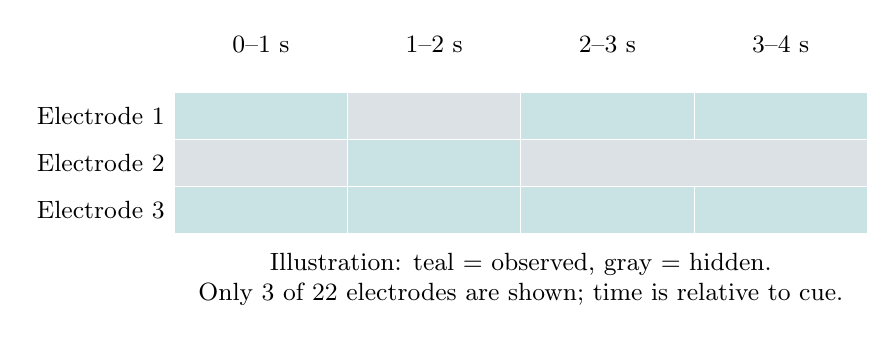
\begin{tikzpicture}[x=22mm,y=6mm,font=\small]
\foreach \p/\lab in {0/{0--1 s},1/{1--2 s},2/{2--3 s},3/{3--4 s}}{
  \node at (\p+.5,1){\lab};}
\foreach \c in {1,2,3}{\node[left] at (0,-\c+.5){Electrode \c};}
\foreach \p in {0,...,3}{\foreach \c in {1,...,3}{
  \filldraw[fill=teal!22,draw=white] (\p,-\c) rectangle (\p+1,-\c+1);}}
\filldraw[fill=graycell,draw=white] (1,-1) rectangle (2,0);
\filldraw[fill=graycell,draw=white] (0,-2) rectangle (1,-1);
\filldraw[fill=graycell,draw=white] (2,-2) rectangle (4,-1);
\node[below,align=center] at (2,-3.2){Illustration: teal = observed, gray = hidden.\\Only 3 of 22 electrodes are shown; time is relative to cue.};
\end{tikzpicture}
\end{center}
\textbf{Full training} uses all 22 electrodes. \textbf{Mixed training} chooses
22, 16, or 6 retained electrodes uniformly per trial each epoch. For 16/6, it
chooses static or dynamic random loss equally. Electrode IDs never shift and no
window may lose every electrode. The model's convolutions may mix channels and
windows \emph{after} hidden values have been removed.

\newpage
\section{The current EEGNet classifier}
EEGNet uses temporal, depthwise spatial, and separable convolutions
\cite{eegnet}. This implementation is an architecture reproduction; its data
split and preprocessing do not reproduce a paper's complete benchmark protocol.

\subsection*{Follow the dimensions through the network}
The four windows are joined back into 1000 time samples after masking. The
extra dimension of size 1 below is an input feature-map axis. $B$ is batch size.

\begin{tabularx}{\linewidth}{@{}L{40mm}L{33mm}Y@{}}
\toprule
Operation & Output shape & What it learns or does \\
\midrule
Masked input & $B\times1\times22\times1000$ & Preserves the original channel order \\
Temporal convolution; BatchNorm & $B\times8\times22\times1000$ & Eight length-64 temporal filters, separately at each electrode \\
Depthwise spatial convolution; BatchNorm; ELU & $B\times16\times1\times1000$ & Two spatial filters per temporal feature, spanning all 22 electrodes \\
Average pooling by 4; dropout & $B\times16\times1\times250$ & Reduces temporal length; dropout rate 0.5 \\
Separable convolution; BatchNorm; ELU & $B\times16\times1\times250$ & Length-16 depthwise temporal filters and pointwise feature mixing \\
Average pooling by 8; dropout & $B\times16\times1\times31$ & Keeps 31 ordered temporal bins; dropout rate 0.5 \\
Flatten & $B\times496$ & $16\cdot31$ values, preserving bin order \\
Optional mask concatenation & $B\times584$ & Adds $22\cdot4=88$ availability flags \\
Linear classifier & $B\times4$ & Four scores, called logits \\
\bottomrule
\end{tabularx}

\textbf{Reference EEGNet} uses the 496 signal features alone.
\textbf{Mask-conditioned EEGNet} also receives the 88 mask flags. Even the
reference receives a mask for removing hidden samples; ``reference'' means it
does not append those flags to the classifier. Neither version needs attention.

\subsection*{The declared comparison has four arms}
\begin{tabularx}{\linewidth}{@{}YL{32mm}L{39mm}@{}}
\toprule
Model & Training input & Evaluation coverage \\
\midrule
EEGNet reference & Full & Full and electrode loss \\
Mask-conditioned EEGNet & Full & Full and electrode loss \\
Mask-conditioned EEGNet & Mixed & Full and electrode loss \\
Covariance + logistic regression & Full & Full only \\
\bottomrule
\end{tabularx}
There are $9\text{ participants}\times3\text{ seeds}\times4\text{ arms}=108$
fits. These are separate participant-specific models, not one network trained
jointly on all participants.

\textbf{Why include covariance?} It supplies a simpler reference. Each filtered,
unnormalized trial yields a $22\times22$ shrinkage covariance matrix. Its matrix
logarithm is vectorized into 253 upper-triangle features, with off-diagonal
entries weighted by $\sqrt2$. A training-fitted feature scaler and logistic
classifier then predict the label. This is a log-Euclidean method; there is no
neural encoder or tensor completion in this arm.

\newpage
\section{What loss trains the neural network?}
\subsection*{From logits to probabilities}
The network outputs four real numbers $z_{ik}$ for trial $i$. Softmax turns them
into probabilities:
\[
p_{ik}=\frac{\exp(z_{ik})}{\sum_{j=0}^{3}\exp(z_{ij})},
\qquad \widehat y_i=\operatorname*{arg\,max}_{k\in\{0,1,2,3\}}p_{ik}.
\]
The predicted class is the largest probability. During training, the loss uses
the probability of the \emph{true} class, even when that class is not the largest.

\subsection*{Cross-entropy is the current baseline's training objective}
For a minibatch $\mathcal B$ with true labels $y_i$:
\[
\boxed{\quad \mathcal L_{\mathrm{CE}}(\theta)
 =-\frac{1}{|\mathcal B|}\sum_{i\in\mathcal B}
 \log p_{i,y_i},\qquad
 z_i=f_\theta(\widetilde X_i,M_i).\quad}
\]
For the reference model, $M_i$ controls input masking but is not concatenated
to the final features. The code passes \emph{logits} directly to
\code{cross_entropy}, which performs the stable log-softmax calculation.
The baseline uses unweighted cross-entropy: no class weights, focal term,
reconstruction loss, or explicit tensor penalty.

\takeaway{\textbf{Numerical example.} If the true class is left hand and the model
assigns it probability 0.70, that trial's loss is $-\log(0.70)\approx0.357$.
At probability 0.25 it is $1.386$; at 0.05 it is $2.996$. Confidently missing
the true class produces a larger penalty. These are illustrative probabilities,
not recorded results.}

For a logit $z_{ik}$, the minibatch derivative is
\[
\frac{\partial\mathcal L_{\mathrm{CE}}}{\partial z_{ik}}
=\frac{p_{ik}-\mathbf1[k=y_i]}{|\mathcal B|}.
\]
Backpropagation carries this signal through the linear classifier and all
convolutions. Thus the features are learned for classification, not frozen in
advance. Full and mixed training use the same loss; only input masks differ.

\subsection*{How parameters are updated}
An epoch is one pass through training trials; each minibatch supplies one update.

\begin{tabularx}{\linewidth}{@{}L{52mm}Y@{}}
\toprule
Setting & Declared baseline value \\
\midrule
Optimizer / minibatch & AdamW / 32 trials \\
Learning rate & Base $10^{-3}$; 10-epoch warmup then cosine decay \\
Weight decay & $10^{-4}$, applied by AdamW separately from the CE value \\
Gradient clipping & Global gradient norm at most 1 \\
Weight constraints & Spatial filter max-norm 1.0; final classifier max-norm 0.25 \\
Training budget & At most 250 epochs; early stopping eligible after 75 \\
Patience & Stop after 50 epochs without a better validation selection score \\
\bottomrule
\end{tabularx}
Dropout and BatchNorm use training behavior during optimization. Validation
uses evaluation mode. AdamW weight decay and max-norm constraints regularize
parameters; they are not additional terms in the reported cross-entropy loss.

\newpage
\section{Training, model selection, and final evaluation}
\subsection*{Three data roles and three different quantities}
\begin{tabularx}{\linewidth}{@{}L{29mm}YY@{}}
\toprule
Partition & What happens & What it must not do \\
\midrule
Training & Fit normalization statistics; fit model parameters by minimizing CE & Use validation/test statistics for fitting \\
Validation & Select the epoch by balanced accuracy; log-loss breaks ties & Backpropagate through validation examples \\
Test & Score the restored selected checkpoint & Select epochs, ranks, or architecture \\
\bottomrule
\end{tabularx}

The selected checkpoint is the epoch with the largest full-input validation
balanced accuracy; a smaller validation log-loss wins a tie. Exact ties keep
the earlier epoch. The final epoch is not necessarily the selected epoch.
\[
\mathrm{BA}=\frac14\sum_{k=0}^{3}
 \frac{\#\{i:y_i=k,\,\widehat y_i=k\}}{\#\{i:y_i=k\}},\qquad
\mathrm{LogLoss}=-\frac1N\sum_i\log p_{i,y_i}.
\]
Balanced accuracy gives each class equal weight, even when artifact removal
changes class counts. Accuracy is the fraction of all correct trials. Neither
accuracy nor balanced accuracy is the differentiable training loss.

\subsection*{One participant and seed, from start to finish}
\begin{enumerate}
\item Load accepted trials, persist the split, and fit training normalization.
\item Initialize one arm with its declared seed. Train minibatches and compute
validation scores after each epoch.
\item Save the best weights, constructor settings, normalization, class/channel
order, and provenance. Restore and verify the saved checkpoint.
\item Freeze that selected model and score full and degraded input conditions.
Run the other arms using matched splits, trial identities, and evaluation masks.
\end{enumerate}

\subsection*{What electrode-loss evaluation measures}
For neural arms, evaluate 22, 16, 11, and 6 retained electrodes. At each degraded
count use static random, static spatial, dynamic random, and dynamic spatial
loss. Static loss keeps one subset throughout a trial. Dynamic loss uses the
four-window schedule A--B--A--A, so some electrodes disappear and return.
Spatial patterns remove spatially structured subsets using fixed schematic
electrode coordinates.

There are five repeats per degraded condition: $1+3\cdot4\cdot5=61$ mask
conditions per partition and neural arm. The covariance reference has only
full-input coverage. Eleven-channel and spatial-loss conditions are evaluation
only. Banks are paired across arms, and nonfull channel subsets are allocated
to separate training, validation, and test partitions.

\textbf{Aggregation:} average mask repeats within a condition, then seeds within
each participant, then participants equally. Keep conditions distinct; report
missing results rather than silently averaging a smaller cohort.

\takeaway{\textbf{Optional robust selection is a different declared policy.}
The baseline package can instead average validation BA over full input and
static/dynamic random loss at 16/6 electrodes. The reproducible baseline in this
guide uses \emph{full-input selection}. Do not confuse it with the completed
tensor follow-up, which used its own declared robust validation rule.}

\newpage
\section{Where tensors enter, and why their loss is separate}
\subsection*{The earlier frozen-feature pipeline on our branch}
Its stages are: train a channel/window-local encoder with a full-input
multi-head attention (MHA) head
using CE; select it on full validation; freeze it; fit training-only feature
normalization and Tucker factors; then train separate attention classifiers
using CE. Freezing disables encoder dropout and BatchNorm updates.

The encoder produces $H\in\mathbb R^{B\times22\times4\times32}$. For one
trial/window, write $H_p\in\mathbb R^{22\times F}$, with $F=32$. Tucker-2 uses
\[
H_p\approx U G_p V^\top,\quad
U\in\mathbb R^{22\times r_c},\quad V\in\mathbb R^{F\times r_f},\quad
G_p\in\mathbb R^{r_c\times r_f}.
\]
Here $U,V$ are shared factors; each trial/window has its own core $G_p$.
Default legacy ranks are $r_c=r_f=4$. The window axis is retained.

\subsection*{Unsupervised reconstruction and the masked ridge solve}
For observed electrodes $\Omega_p$, $n_p=|\Omega_p|$, and ridge $\lambda=10^{-3}$:
\[
\mathcal J_p(G_p;U,V)=
\frac{1}{n_p F}\sum_{c\in\Omega_p}\sum_{f=1}^{F}
 \big[H_{pcf}-(UG_pV^\top)_{cf}\big]^2
 +\lambda\lVert G_p\rVert_F^2.
\]
Factor fitting averages this objective over training trials/windows. It alternates
core solves with Adam updates of $U,V$, normalizing each factor column to unit
length. It does not use class labels. Fitted factors then become frozen buffers.
For each new masked input, solve for its core using observed values only:
\[
(U_{\Omega_p}^{\top}U_{\Omega_p})G_p(V^\top V)
 +(n_pF\lambda)G_p=U_{\Omega_p}^{\top}H_{p,\Omega_p}V.
\]
The factor $n_pF$ follows from averaging squared error over observed entries.
Positive ridge makes the conditional core unique; it does not guarantee recovery
of missing signal or preservation of class information.

\textbf{Core classification} feeds $G_p$ to a classifier.
\textbf{Completion} keeps observed entries exactly and replaces only missing
ones by $UG_pV^\top$. Both then train their classifier using CE with factors
fixed. \textbf{There is no jointly optimized CE-plus-reconstruction loss} in
this staged design. Better reconstruction need not mean better classification.

\subsection*{George's separate raw-completion design}
At \code{origin/main} revision \code{92b7fc2}, the tensor input is normalized
\emph{raw} windows, so $F=250$, $r_c=4$, and $r_f=16$. Training-only factor
fitting precedes an end-to-end EEGNet or Signal Transformer with built-in MHA.
Both backbones train on full inputs using CE. Completion is bypassed for full
input, and fills missing raw values only during degraded evaluation. This is
a different experiment from the frozen-feature comparison.

\takeaway{\textbf{A possible future controlled test:} use one selected, strong
EEGNet checkpoint and compare zero-fill with training-fitted raw completion under
the same masks. This is a proposed next experiment, not the current baseline
implementation or an established accuracy improvement.}

\newpage
\section{How to connect this guide to the repository}
\subsection*{Files that define the current baseline}
\begin{tabularx}{\linewidth}{@{}L{73mm}Y@{}}
\toprule
File & Responsibility \\
\midrule
\code{configs/baselines-reproducible.json} & Declared participants, arms, split, and training settings \\
\code{inm/data.py} & GDF cues, exclusions, and window-local filtering \\
\code{agfl/datasets/splits.py} & Persisted trial partitions \\
\code{inm/baselines/data.py} & Training normalization and prepared trial data \\
\code{inm/availability.py} & Electrode identities and paired availability masks \\
\code{inm/baselines/eegnet.py} & Raw masking and the EEGNet architecture \\
\code{agfl/optimization.py} & Cross-entropy implementation \\
\code{inm/baselines/training.py} & AdamW, validation selection, checkpoint saving/reloading \\
\code{inm/baselines/covariance.py} & Log-covariance and logistic reference \\
\code{inm/baselines/reporting.py} & Coverage checks and hierarchical aggregation \\
\code{inm/tensor_attention.py} & Earlier Tucker objective and masked core solve \\
\bottomrule
\end{tabularx}

The covariance arm minimizes a multinomial logistic classification objective
with L2 regularization ($C=1$), using L-BFGS with at most 1000 iterations. It
does not use the neural epoch schedule. Its feature scaler and classifier are
fitted on training data; its covariance calculation is performed per trial.

\subsection*{Inspect a plan without launching training}
From the repository root:
\begin{quote}\small
\begin{verbatim}
python -m inm.baselines \
  --config configs/baselines-reproducible.json --plan
\end{verbatim}
\end{quote}
This prints 27 participant/seed tasks and 108 fits. By contrast,
\texttt{python run.py -{}-plan} describes the earlier experiment: 27 tasks and
378 classifier fits. They are different entry points and different protocols.

\subsection*{What remains a research question}
Our current priority is to understand training and validation behavior of the
spatial EEGNet baseline before adding complexity. A high training score and
lower validation score should prompt checks of generalization, trial alignment,
and preprocessing. They do not by themselves identify the cause.

This document explains source behavior, not a new experiment. No training was
run to produce it. Existing empirical reviews are in \code{docs/baselines/};
the branch comparison is \code{docs/baselines/branch-review.md}. The older
\code{agfl_concept.pdf} remains a detailed companion for the frozen-feature
tensor mathematics. Changed source, packages, or experiment settings require a
new result directory with its own provenance.

\begin{thebibliography}{9}\small
\bibitem{dataset} C. Brunner et al. \emph{BCI Competition 2008, Graz data set A}
(BCI Competition IV, dataset 2a). Official recording and task description.
\url{https://www.bbci.de/competition/iv/desc_2a.pdf}.
\bibitem{eegnet} V. J. Lawhern et al. \emph{EEGNet: A Compact Convolutional
Network for EEG-based Brain-Computer Interfaces}. 2018.
\url{https://arxiv.org/abs/1611.08024}.
\end{thebibliography}
\end{document}
